\chapter{Semi-analytical model for beam dynamics} 
% Previous models, bonatto 
%All assume static beam and unchanging density of both beam and plasma, up until the point of saturation
%We present a model here that make accurate predictions, not only past the point of saturations but also includes densty variations and even predicts the energy of the ejected particles
The details of PIC codes was described in detail in the previous report, see chapter 2 of the previous report for further details. Conventional PIC codes will simulate millions of macroparticles and update all their positions while considering their mutual Coloumb interactions. These also include collisions effects, ionisation, synchrotron and bremsstralung and many additional physical effect. For our purposes however we simply want a quick model to give us a rough idea of the behaviour of these varying density schemes that we are considering. 
\section{Single-particle dynamics}
\subsection{Longitudinal and transverse wakefields}
The equations governing the behaviour of the plasma under the influence of an electron beam were derived from first principles in the previous report. We include them below in the form most commonly used in today's literature. 
The angular plasma frequency
\begin{equation}
\label{PlasmaFrequency}
\omega_{p}=\sqrt{\frac{4 \pi e^{2} n_{p}}{m_{e}}}
\end{equation}
gives the frequency of oscillations of the plasma waves as a beam passes through the plasma. The longitudinal force can be shown to be given by 
\begin{equation}
\label{LongitduinalIntegral}
 \frac{E_{z b}(\xi, r)}{E_{0}}=-k_{p}^{3} \int_{\infty}^{\xi} d \xi^{\prime} \cos \left[k_{p}\left(\xi-\xi^{\prime}\right)\right]  \int_{0}^{\infty} d r^{\prime} r^{\prime} I_{0}\left(k_{p} r_{<}\right) K_{0}\left(k_{p} r_{>}\right) n_{b}\left(\xi^{\prime}, r^{\prime}\right) / n_{0} 
\end{equation}
where $k_p=\omega_p/c$ is the plasma wavenumber. The longitudinal (displacement variable)/(convolution variable) $\xi'$ in our Green's function is integrated across the interval $\xi'\in[\infty, \xi]$ to emphasise the fact that the wakefield at a position $\xi$ behind the beam can only be caused by interactions of particles in front of that positions due to causality.
The Panofsky-Wenzel theorem states that the transverse field corresponding to a given longitudinal field is given by
\begin{equation}
\label{Panofsky-Wenzel}
W\left(\xi,r\right)=\int^{\xi}_{\infty}\frac{\partial E_z\left(\xi,r,z\right)}{\partial r}\mathrm{d}\xi
\end{equation}
which upon differentiation and integration yields
\begin{equation}
\label{transverseIntegral}
\frac{W_{\perp}(\xi,r)}{E_{0}}=-k_{p}^{3} \int_{\infty}^{\xi} \sin \left(k_{p}\left(\xi-\xi^{\prime}\right)\right) \mathrm{d} \xi^{\prime} \int_{0}^{\infty} \frac{\partial}{\partial r}\left(I_{0}\left(k_{p} r_{<}\right) K_{0}\left(k_{p} r_{>}\right)\right) \frac{n_{b}\left(\xi^{\prime},r^{\prime}\right)/n_0}{\partial r^{\prime}} r^{\prime} \mathrm{d} r^{\prime}
\end{equation}
Since the aim of this model is to model the beam dynamics in a varying plasma density we need to include its effect on the induced wakefield, as described by equations \ref{LongitduinalIntegral} and \ref{transverseIntegral}. The plasma density only enters the above equations through the wavenumber $k_p$, which both scales the overall amplitude of the wakefield as well as determines the rate of oscillations and decay of the wakefield through its inclusion in the trigonometric and Bessel functions, respectively. Hence by letting the plasma density $n_p\mapsto n_p(z)$ as a function of the propagation distance $z$ the wavenumber will vary at each longitudinal position as well, $k_p\mapsto k_p(z)$, which in turn adds a propagation distance dependence in the wakefield equations: $E_{z}(\xi,r,z)$ and $W_{\perp}(\xi,r,z)$. These expressions can be solved numerically in software such as Mathematica, but the calculation is time-consuming and often approximations are used. Before going into detail about how we approximate and  compute these expressions it is necessary to describe the algorithm in which aim to use them to understand the degree of approximation necessary. 
\subsection{Particle-push algorithm}
The first simplification used in this algortihm is to condisder the dynamics of a test particle inside the bunch under the influence of the wakeifeld set up by the electron bunch as it propagates through a plasma. We assume that the shape and density of the beam is static as it propagates through the plasma, thereby removing the need to constantly having to update the beam density $n_b$ in the wakefield integrals. Furthermore, we assume that the only forces acting on the test-particle are the electric fields of the wakefields themselves, thereby ignoring the Coulomb repulsions within the bunch, synchrotron and betatron radiation etc. Hence to determine the dynamics of we simply need to place it at a position $(\xi_i,r_i)$ inside the bunch and its wakefield, with an energy equal to that of the particle in the bunch, and calculate the forces acting on it at that positions. Then, by choosing a sufficiently short time-step $\Delta t$ that we allow these forces to act on the particle, we can calculate a new positions $(\xi_{i+1},r_{i+1})$ that the particle will have moved to during this time. By repeating this process we should be able to determine how this particle will behave as it gets decelerated and falls behind the bunch. By further increasing the density at each iteration we should be able to investigate what happens when this particle enters the defocusing region.\\
\indent This approach is inspired by the particle-push and field-solver algorithms underlying all PIC codes. These algorithms, described in detail in chapter 2 of the previous report, only act as inspiration for this model and are not necessary to understand this model. The method by which we perform the iterations in this algorithm are described in this section.\\
Firstly, a position $(\xi_{0},r_{0})$ inside the bunch is chosen as a starting point for our test particle. The energy of this particle is then set to equal that of the particles in the beam, e.g 1 GeV to allow for comparison with the simulations in chapter 2. We then set the size of the time-step $\Delta t$ used to discretize the particle motion. To calculate the particles new position $(\xi_{1},r_{1})$ after time $\Delta t$, or more generally any new position $(\xi_{i+1},r_{i+1})$ given a current position $(\xi_{i},r_{i})$, we first need to calculate the longitudinal and transverse electric field at this position, $E_{z}(\xi_i,r_i,z)$ and $W_{\perp}(\xi_i,r_i,z)$, where $z$, the distance the beam has travelled through the plasma $z=i\cdot v_{beam}\Delta t$ is used to determine the density at that position given a density profile $n_p(z)$. The speed $v_{beam}$ of the particles in the ultra-relativistic beam is given by kinetic energy $T_{beam}=(\gamma-1)m_ec^2$ as
\begin{equation}
v_{beam}=c \sqrt{1-\left({1+\frac{T_{beam}}{m_ec^2}}\right)^{-2}}
\end{equation}
which is very close to the speed of light for our 1 GeV bunch, but nevertheless must be calculated as it is crucial for subsequent steps of the algorithm.
The same equation can be used to updated the longitudinal speed of the test particle from $v_z(i)$ to $v_z(i+1)$ if the updated kinetic $T_e(i+1)=T_e(i)+\Delta T_e(i)$ can be found. The kinetic energy change of the particle $\Delta T_e(i)=T_e(i+1)-T_e(i)$ between iterations $i$ and $i+1$ is given by work done on the particle by the longitudinal wakefield during time $\Delta t$. This work, in turn, is given by integrating the force exerted on the particle over the distance $v_z(i)\Delta t$ that the particle moves during the iteration. However, since we assume that the force is constant in each iteration we have that
 %Similarly, the longitudinal speed of the test particle at position iteration $i+1$ is given by it's kinetic energy $T_e(i+1)=$ through
\begin{equation}
\Delta T_e(i)=-eE_z\left(\xi_i,r_i,z_i\right) v_z(i)\Delta t
\end{equation} 
which we use to updated the longitudinal speed to
\begin{equation}
v_z(i+1)=c \sqrt{1-\left({1+\frac{T_e(i)+\Delta T_e(i)}{m_ec^2}}\right)^{-2}}
\end{equation}
Even though reference is made to the co-moving variable $\xi$ in the above calculation, the calculation itself is performed in the lab frame where the beam has an energy of 1 GeV etc. However, to calculate at what longitudinal position $\xi_{i+1}$ , with respect to the beam and its wakefield, the particle will end up after time $\Delta t$ we now move into the co-moving reference frame. Given that we know the force acting on the particle and the initial velocity, the updated position is given by relativistic equivalent of the standard $x=vt+at^2/2$ formula. From relativistic kinematics we found that this is given by
\begin{equation}
\label{XiUpdate}
 \xi_{i+1}=\xi_i + \frac{v_z(i)-v_0}{1-v_z(i)v_0/c^2}\Delta t -\frac{c^2 }{a_z}\left(1-\sqrt{1+\frac{a_z^2 \Delta t^2}{c^2}}\right)
 \end{equation} 
 where the second term gives the relative velocity $v_{\xi}'$ between the particle and the wakefield in the co-moving frame and $a_z$ is the acceleration in the longitudinal direction. If the particle is moving relativistic in co-moving frame, i.e when falling behind the bunch the speed of the particle relative to the wakefield is $-c$, the relativistic acceleration expression needs to be used. The force in the co-moving (primed) frame
 \begin{equation}
 \vec{F}'=\frac{\mathrm{d}\vec{p}'}{\mathrm{d}t}
 \end{equation}
now needs to include the relativistic momentum $\vec{p}'=m_e \gamma( \vec{v}') \vec{v}'$, where $|\vec{v}'|=\sqrt{{v_{\xi}'}^2+v_r^2}$ is the speed of the particle in the co-moving frame, which gives that the acceleration in the co-moving frame
 \begin{equation}
 \vec{a}'=\frac{1}{m_e\gamma(|\vec{v}'|)}\left(\vec{F}'-\frac{(\vec{v}'\cdot\vec{F}')\vec{v}'}{c^2}\right)
 \end{equation}
 Taking the longitudinal component of this then gives the longitudinal relativistic acceleration
 \begin{equation}
 a_z(i)=-\frac{eE_z\left(\xi,r,z\right)}{m_e\gamma(|\vec{v}'|)^3}
 \end{equation}
which due to the gamma term is only of concern when the relative velocity between particle and wakefield in the co-moving frame is large. Using this expression in equation \ref{XiUpdate} we now update the co-moving position to $\xi_{i+1}$, thereby completing the longitudinal push. 

Due to the rapid variation in the radial position and velocity the kinetic energy approach has proven inaccurate for too long time steps, since vr might be negative in one iteration and positive in the next, providing inaccurate descriptions of the distance the transverse wakefield has exerted force on the electron.  For this reason we compute the  
\begin{equation}
\Delta v_r(i)=\frac{a_r(i) \Delta t}{\sqrt{1+\frac{a_r^2(i) \Delta t^2}{c^2}}}
\end{equation}
where the transverse acceleration is given by the transverse component of equation XX.
 \begin{equation}
 a_z(i)=-\frac{eE_z\left(\xi_i,r_i,z_i\right)}{m_e\gamma(|\vec{v}'|)^3}
 \end{equation}
and the updated velocity is given by relativistic velocity addition
\begin{equation}
v_r(i+1)=\frac{v_r(i)+\Delta v_r(i)}{\sqrt{1+\frac{v_r(i)\Delta v_r(i)}{c^2}}}
\end{equation}
The updated radial positions is then given by the radial equivalence of equation XX. 
\begin{equation}
\label{RUpdate}
r_{i+1}=r_i+v_r(i)\Delta_t -\frac{c^2}{a_r(i)} \left(1-\sqrt{1+\frac{a_r^2(i) \Delta_t^2}{c^2}}\right)
\end{equation}
%where the relativistic formula ensures that large accelerations do not correspond to  displacements violating causality.
By placing a test particle at positions in the beam we can then track the behaviour of this particle under the influence of the wakefield described by the the linear fluid model as the density changes. This of course neglects all Coloumb repulsion for particles in the beam, synchrotron radiation emission etc. 
However, to model the dynamics of this particle under the extremely strong electric field set up by the wakefield one needs to use a small step size in the algortihm to avoid pushing the particle too far or accelrating it for too long. To calcualte these forces the wakefield integrals need to be solved at each iteration step, which is a computationally expensive procedure that would ultimately ruin this algorithm if not simplified substantially.
\subsection{Semi-analytical model}
In order to calculate the wakefield induced by a bi-Gaussian beam with density
\begin{equation}
\label{BigaussianBeamDensity}
n_b(\xi,r)= n_{b_0}e^{-\frac{\xi ^2}{2 \sigma{_\xi}^2}-\frac{r ^2}{2 \sigma_r ^2}}
\end{equation}
we need to compute the wakefield integrals \ref{LongitduinalIntegral} and \ref{transverseIntegral}. These integral can be separated into integration over the co-moving variable $\xi$ and the radial distance $r$. For a Gaussian beam a closed form expression for the $\xi$ integral in equation \ref{LongitduinalIntegral} can be found
\begin{equation}
\label{Ezxi}
\begin{aligned}
E_{z b}(\xi)&= \int_{\infty}^{\xi} d \xi^{\prime} \cos \left[k_{p}\left(\xi-\xi^{\prime}\right)\right] e^{-\frac{\xi'^2}{2 \sigma{_\xi}^2}} \\
 &= \frac{1}{2} \sqrt{\frac{\pi }{2}} k_pn_{b_0} \sigma{_\xi}  e^{-\frac{1}{2} k_p \left(k_p\sigma{_\xi}^2+2 i \xi \right)}
   \left(\text{erfc}\left(\frac{\xi -i k_p\sigma{_\xi}^2}{\sqrt{2} \sigma{_\xi}}\right)+e^{2 i k_p\xi } \text{erfc}\left(\frac{\xi +i
   k_p\sigma{_\xi}^2}{\sqrt{2} \sigma{_\xi}}\right)\right)
   \end{aligned}
\end{equation}
where, as is often the case for integration involving Gaussians, the complementary error function [ref] 
\begin{equation}
\text{erfc}(x)=\frac{2}{\sqrt{\pi}} \int_{x}^{\infty} e^{-u^{2}} \mathrm{d}u
\end{equation}
appears in the expression. A close form expression is however not possible for the radial integral in equation \ref{LongitduinalIntegral}:
\begin{equation}
\label{Ezr}
 E_{z b}(r)=  \int_{0}^{\infty} d r^{\prime} r^{\prime}\Big[ I_{0}\left(k_{p} r\right) K_{0}\left(k_{p} r'\right)\Theta\left(r'-r\right)  +I_{0}\left(k_{p} r'\right) K_{0}\left(k_{p} r\right)\Theta\left(r-r'\right)     \Big]e^{-\frac{r ^2}{2 \sigma_r ^2}}
\end{equation}
since the convolution of the modified Bessel functions with the Gaussian radial function can only be evaluated numerically, at least as far as the author is aware. To achieve a closed form expression of this integral we approximate the radial Gaussian by expanding it to second order such that
\begin{equation}
n_b(r)=\left(1-\frac{r^2}{2 \text{$\sigma $r}^2}\right) \theta \left(\sqrt{2} \text{$\sigma $r}-r\right) + \mathcal{O}\left(r^4\right)
\end{equation}
where the Heavieside function $\theta \left(\sqrt{2} \sigma_r-r\right)$ prevents negative densities. This approximation yields a closed form expression when evaluated in equation \ref{Ezr}, which we then multiply by expression \ref{Ezxi} as well as add a density-profile dependence to the plasma wavenumber, $k_p\mapsto k_p(z)$,  to give our approximate longitudinal wakefield:
\begin{equation}
\label{EzApprox}
\begin{split}
E_z\left(\xi,r,z\right)&=\frac{1}{2} \sqrt{\frac{\pi }{2}} k_p^3(z) n_{b_0} \sigma_{\xi}  e^{-\frac{1}{2} k_p(z) \left(k_p(z) \sigma_{\xi} ^2+2 i \xi \right)}
   \left(\text{erfc}\left(\frac{\xi -i k_p(z) \sigma_{\xi} ^2}{\sqrt{2} \sigma_{\xi} }\right)+e^{2 i k_p(z) \xi } \text{erfc}\left(\frac{\xi +i k_p(z) \sigma_{\xi} ^2}{\sqrt{2} \sigma_{\xi} }\right)\right) \\
   & \left(-\frac{\theta \left(\sqrt{2}\sigma_r-r\right) \left(k_p(z)^2 \left(r^2-2 \sigma_r^2\right)+4
   k_p(z)^2 \sigma_r^2 \left(K_0(k_p(z) r) I_2\left(\sqrt{2} k_p(z) \sigma_r\right)\right)\right)}{2 k_p(z)^4 \sigma_r^2}\right)\\
   & \left(\frac{2 K_0(k_p(z) r) I_2\left(\sqrt{2} k_p(z) \sigma_r\right)}{k_p(z)^2}+\frac{ \left(4
   k_p(z)^2 \sigma_r^2 \left( I_0(k_p(z) r) K_2\left(\sqrt{2}
   k_p(z) \sigma_r\right)\right)+4\right)}{2 k_p(z)^4 \sigma_r^2}\right)
   \end{split}
\end{equation}
where $I_2$ and $K_2$ are the second-order modified Bessel functions of the first and second kind, respectively. To find the transverse wakefield $W_{perp}$ in this approximation we again use the Panofsky-Wenzel theorem and equation \ref{Panofsky-Wenzel}. The full expression is lengthy and contained in Appendix XXX for your amusement. Despite the length and complexity of these expressions, they evaluate significantly faster than the original integrals. Our algorithm can therefore make efficient use of them to allow a a large number of to be performed at a reasonable time. To investigate to what accuracy this model can describe single-particle dynamics inside a wakefield as well as ejection of particles due to defocusing, we set up the model to run with the same partameters as those in simulation XXX of chapter 2. We then place a test particle at a position $\left(\xi=0,r=1\mu \text{m}\right)$ to represent a particle close to the middle of the beam. The radial offset of one micron is chosen to give a non-zero transverse force, which is zero at precisely $r=0$. We also set the kinetic energy of the test particle $T_e(i=0)=1\text{GeV}$. The step-size is set to $\Delta t=1\text{fs}$ which given an electric force on the order of GeV/m corresponds to a particle radial displacement of $<0.1\mu \text{m}$, this ensures that the test particle is not pushed  past the center of the beam in the first iteration, where the transverse force changes direction . We then proceed to iteratively update $\xi_i\to\xi_{i+1}$ and $r_i\to r_{i+1}$ using equations \ref{XiUpdate} and \ref{RUpdate}, respectively. These in turn compute the longitudinal and transverse wakefields using the approximate expressions in equations \ref{EzApprox} and \ref{WApprox}. Finally, we perform run the model using two density profiles: a uniform density, from which we should expect no transverse ejection, and the density profile 
\begin{equation}
n_p(z)=\left\{\begin{aligned} &~~~~~~~n_0~~&&,~~z\leq z_c \\
&n_0\frac{c_1}{(c_2-z)^2}~~&&,~~z>z_c
 \end{aligned}\right.
\end{equation}
which was used in the simulation, such that $k_p(z)$ gets updated after each iteration as described in section 3.1.2 [Particle-push algorithm]. By storing the energy and position of the particle after each iteration we can then plot the trajectory of the particle as it falls behind the beam, the results of which is shown in figure \ref{RadialEjectionModel}. Where we can see that since the test particle starts in a region of focusing field it oscillates around the axis of propagation, until it has fallen behind the beam long enough to reach the defocusing region, where it subsequently gets expelled. [Add stuff about the energy plot and energy of ejected particle]
%Once all approximations are in place, show what happens to particle initially displaced from axis in beam. Show oscillations as it falls behind and gets defocused (maybe show what happens it not defocused as well for uniform plasma )\\
By following a particle through this algorithm all the way until it falls behind the beam and ends up getting defocused, as a result of an increasing density and approaching defocusing region, we can get a prediction of the energy of the ejected 

\begin{figure}
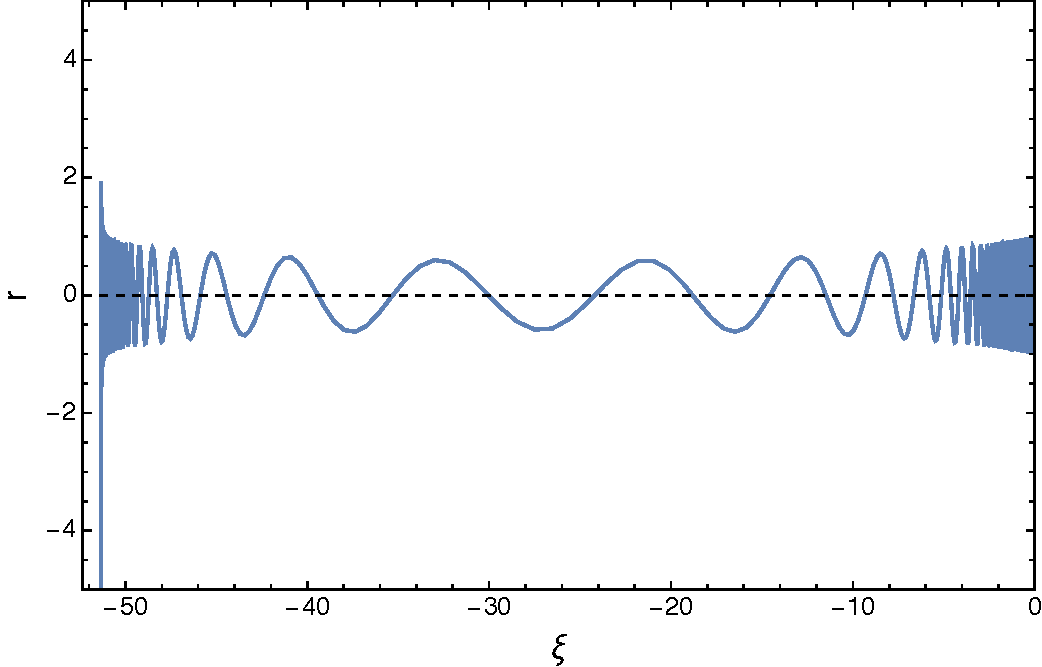
\includegraphics[width=0.8\textwidth]{RadialEjectionFull}
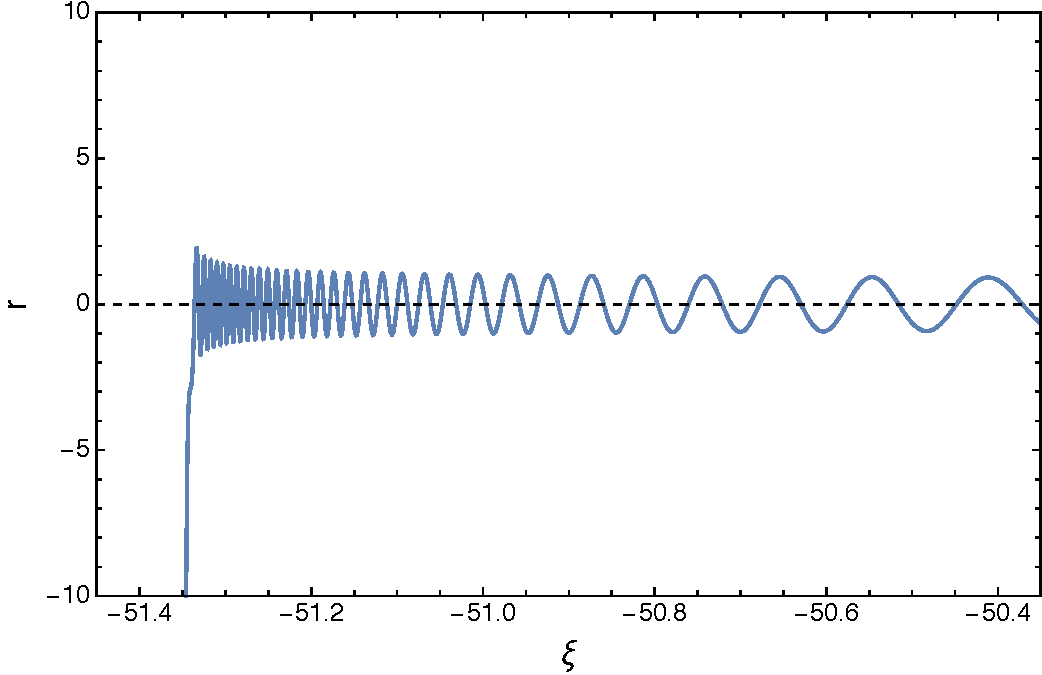
\includegraphics[width=0.8\textwidth]{RadialEjectionZoom}
\caption{Put constant density and increasing density three plots (radialfull, radialzoom,energy) next to each other in two columsn. Maybe re-do in python and overall wakeifled to see how far in defocusing region the particle gets ejected. Add lines on full plot to indicate zoomed in second plot. Also ad plot of kinetic energy above these two.}
\label{RadialEjectionModel}
\end{figure}
[Add plots for different radial starting positions to learn what determines ejection energy after the beam dynamics section instead.]
\section{Beam dynamics}
\subsection{Static beam approximation}
In this section we outline how the model for single-particle dynamics can be extended to extend to model the behaviour of a full beam. This approach assumes that the density of the beam, $n_b(\xi,r)$, used to induce the wakefield is constant as it propagates through the varying plasma density is constant.  Firstly, the single-particle algorithm is run for multiple test particles starting at various positions within the beam. The combined dynamics of these particles can then be used to represent the kinematics of the beam itself. However, before doing so the contribution of each test particle to the beam must be considered. This is because the beam we are modelling is a bi-Gaussian as given by equation \ref{BigaussianBeamDensity}. Consequently, a test particle placed far away from the center of the beam needs to represent fewer electrons in the beam than a test particle close to the center of the beam, where the density is significantly higher. Furthermore, since we want to utilize the cylinidrical symmetry of our equations to the fullest, a test particle at as starting position $(\xi,r)$ should represent all particles at that position around the beam axis. Hence each test particle has an associated volume, given by an annular cross-section of a sphere of circumference $2\pi r$, multiplied by thickness its radial and longitudinal thickness, as shown in figure XXX. The contribution of this volume to the overall beam properties is then weighted in proportion to its placement in the bi-Gaussian beam. 
\begin{figure}
\centering
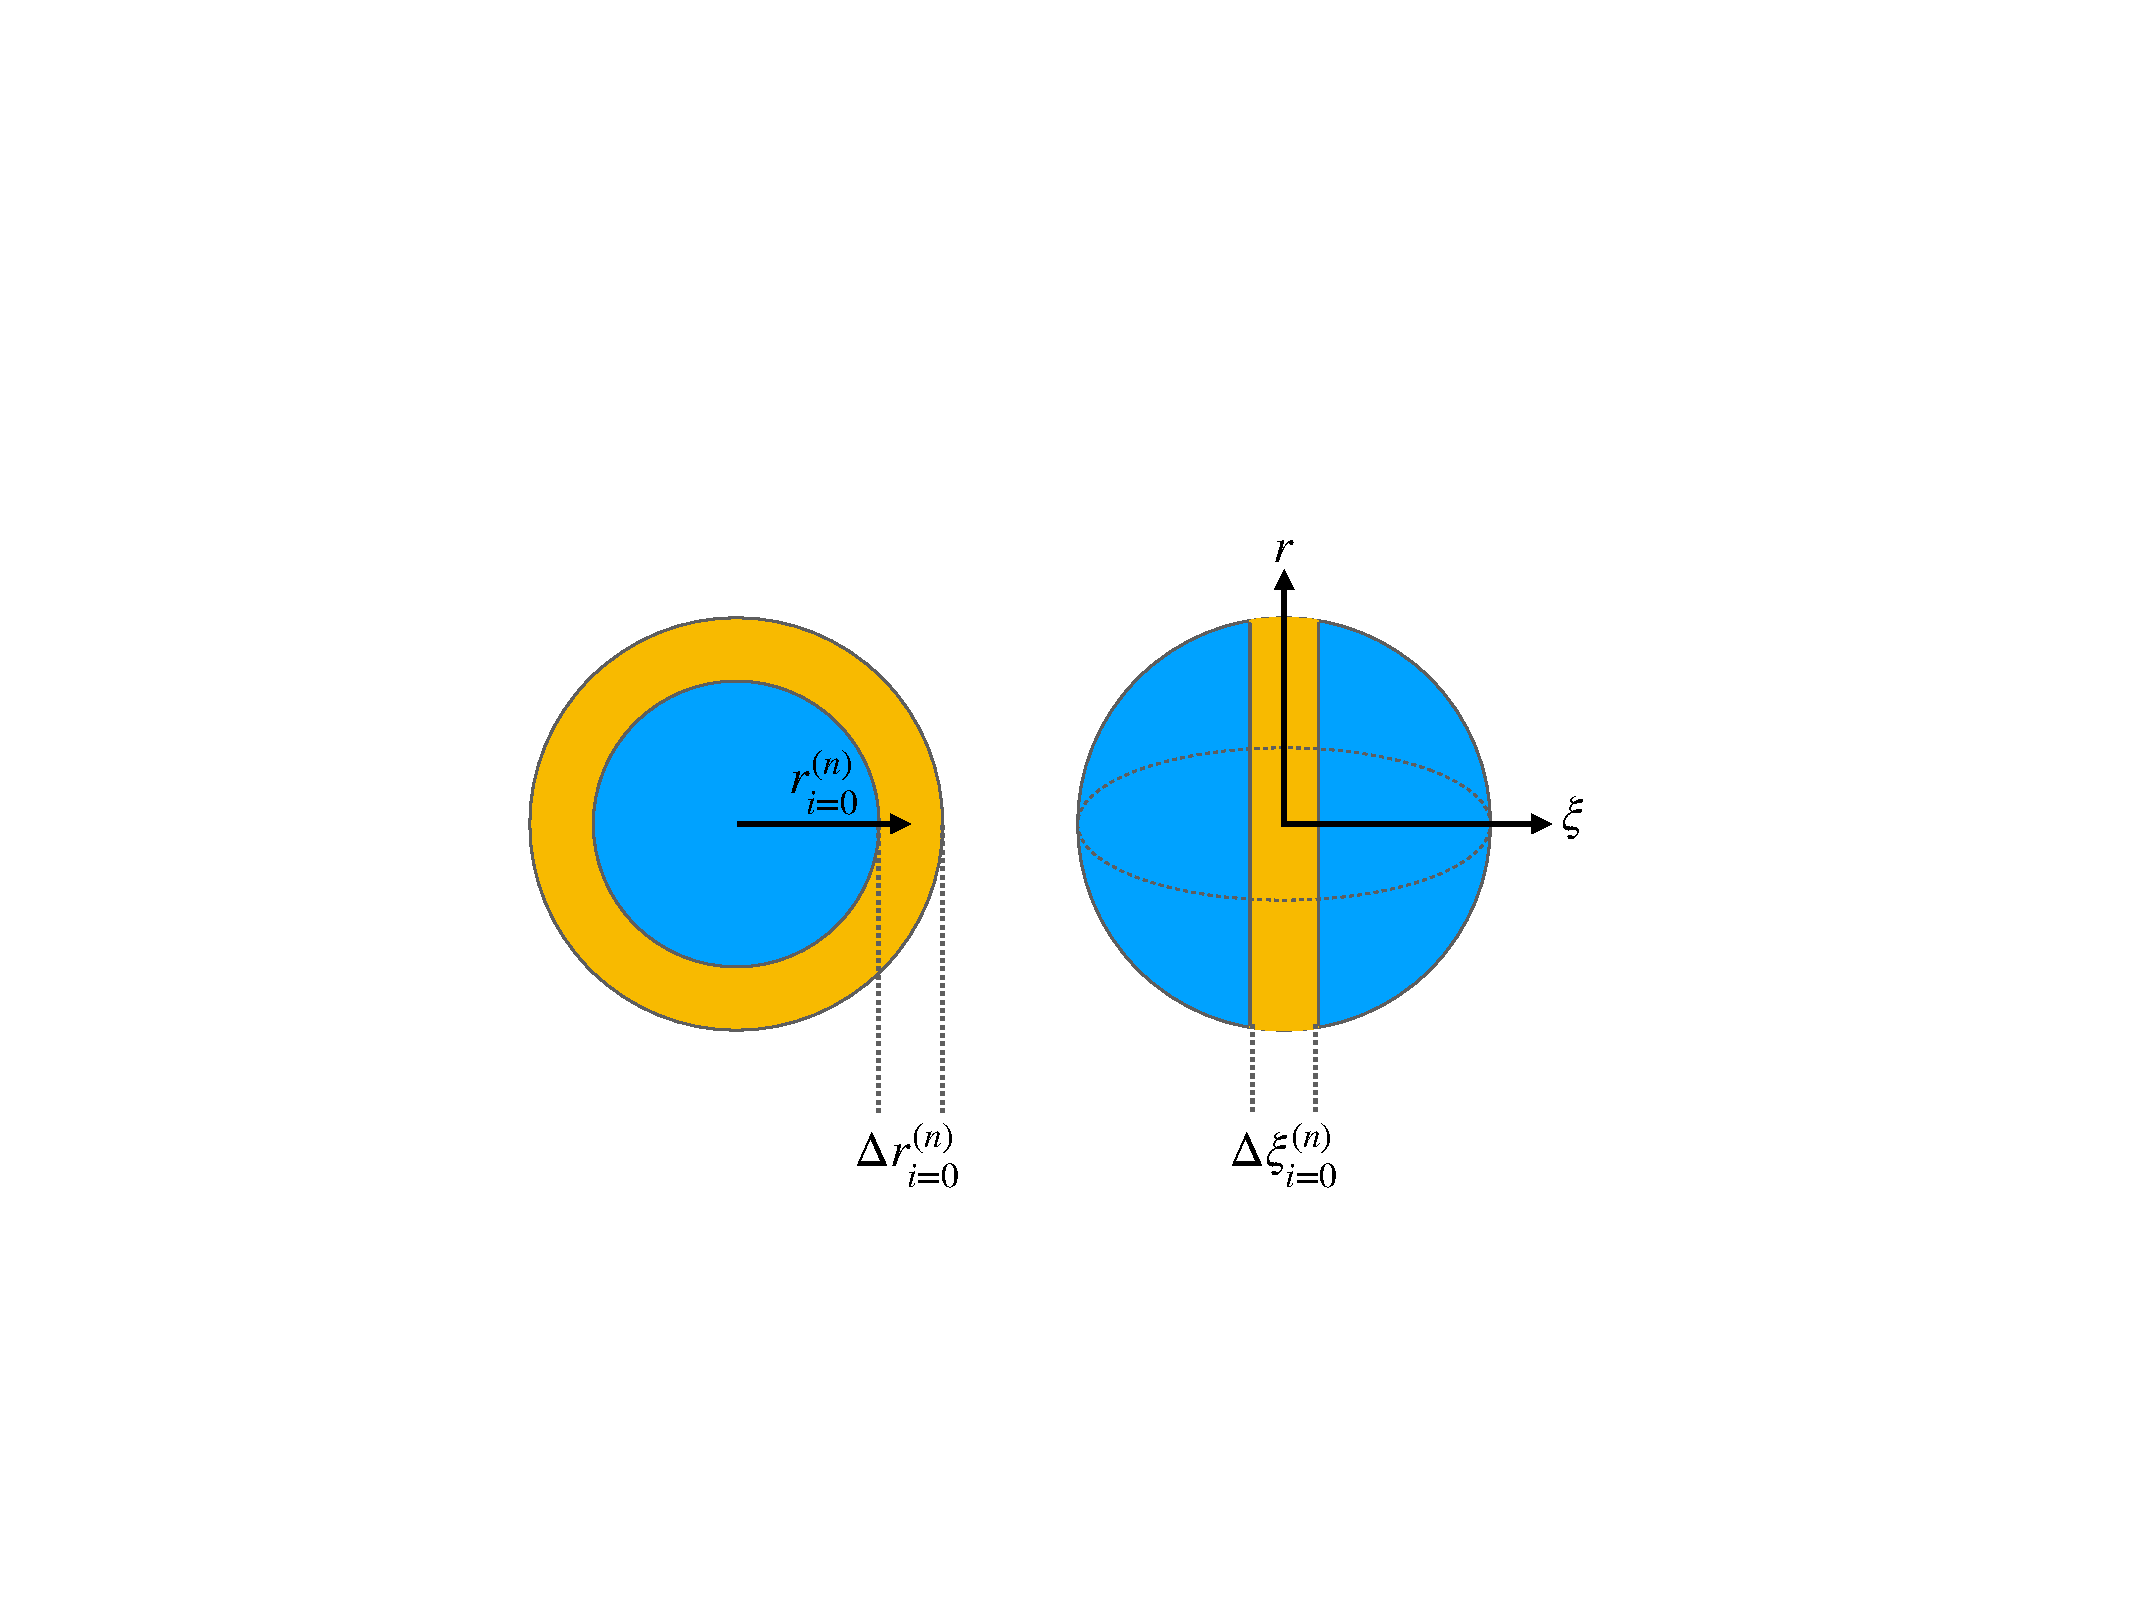
\includegraphics[width=0.6\textwidth]{AnnularCrosssSection}
\end{figure}
With these weighting factors in place we then choose a distribution of test particles evenly along the beam. For instance, by placing test particles in the ranges $-2\sigma_{\xi}\leq\xi\leq 2\sigma_{\xi}$ and $0<r\leq2\sigma_r\leq$ we cover $91.1\%$ of the volume of the bi-Gaussian beam. Having run the single-particle algorithm for these test particles we can then access the energy of the test particle at each propagation distance $z$. These are then summed together and weighted according to their starting positions to give the energy of the pseudo-beam as a function of propagation distance z:
%from -2sigma to +2sigma cover 95 percent of data, however in order use these particles together to represent the dynamics of the beam their contibutions must be weighted with respect to their position. 
\begin{equation}
T_{beam}(z)= \sum_{n=0}^N T_e^{(n)}(z)\times 2\pi r_{i=0}^{(n)}\times\Delta r_{i=0}^{(n)}\times\Delta \xi_{i=0}^{(n)}\times\exp[-\frac{\left(\xi_{i=0}^{(n)}\right)^2}{2\sigma_{\xi}^2}-\frac{\left(r_{i=0}^{(n)}\right)^2}{2\sigma_{r}^2}]
\end{equation}
where $(\xi_{i=0}^{(n)},r_{i=0}^{(n)})$ are the test-particle starting positions, which is weighted by the bi-Gaussian accordingly. The volume of each test particle is given by the circumference of the annular cross section $2\pi r_{i=0}^{(n)}$, multiplied by the radial and longitudinal widths $\Delta r_{i=0}^{(n)}=( r_{i=0}^{(n+1)}-r_{i=0}^{(n)})$ and $\xi_{i=0}^{(n)}=( \xi_{i=0}^{(n+1)}-\xi_{i=0}^{(n)})$, respectively. The kinetic energy of the test particles after each iteration, $T_e^{(n)}(z)$, is set to zero if the particle has been ejected at a position $z_{eject}<z$. Similarly, the total ejected energy can be calculated by storing the position and energy of the particle when it is ejected:
\begin{equation}
E^{Tot}_{eject}(z)=\sum_{n\in n_{eject}(z)} T_e^{(n)}(z_{eject})\times 2\pi r_{i=0}^{(n)}\times\Delta r_{i=0}^{(n)}\times\Delta \xi_{i=0}^{(n)}\times\exp[-\frac{\left(\xi_{i=0}^{(n)}\right)^2}{2\sigma_{\xi}^2}-\frac{\left(r_{i=0}^{(n)}\right)^2}{2\sigma_{r}^2}]
\end{equation}
were $n_{eject}(z)$ is the set of particles ejected at a position $z_{eject}<z$, which are again appropriately weighted by their starting position. It should be emphasized that the thickness $\Delta \xi_{i=0}^{(n)}$ is again given by the difference in position between successive test-particles and not, as the above equation might suggest, by the difference in position between successive ejected test-particles. \\
\begin{figure}
\centering
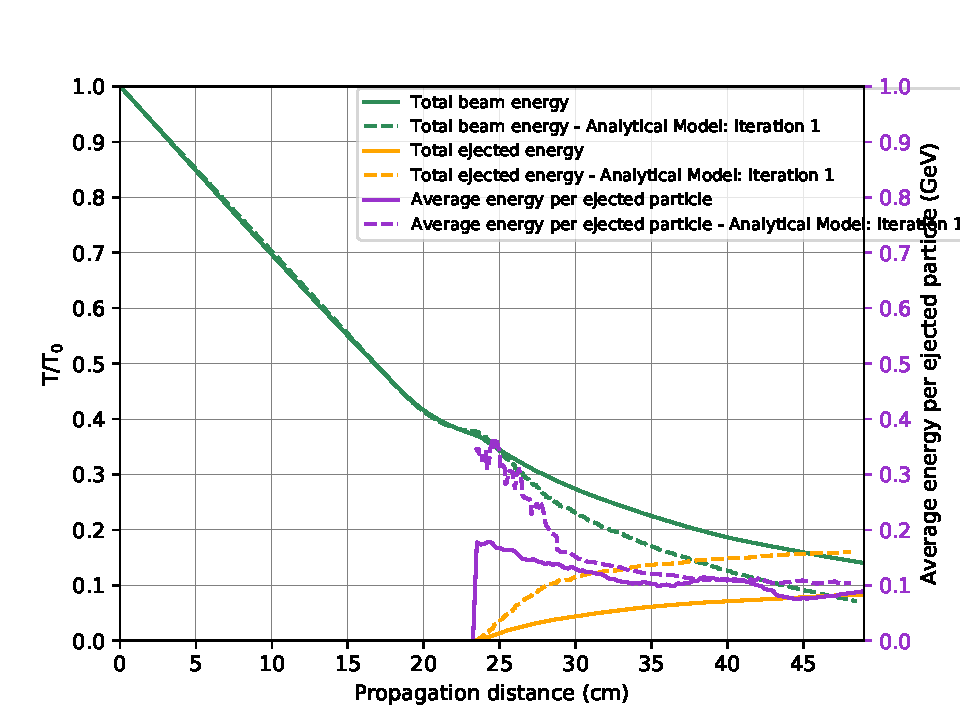
\includegraphics[width=0.8\textwidth]{EnergiesIteration1.pdf}
\caption{Comparison of results for semi-analytical model in the static beam approximation and 2D EPOCH simulation. [Add average energy per ejected particle as well.]}
\label{ConstantPlowIteration1}
\end{figure}
\indent Figure \ref{ConstantPlowIteration1} shows the results for running this model with the same simulation parameters as in figures XXX, using longitudinal and radial starting positions in the range $-2\sigma_{\xi}  \leq  \xi_{i=0}^{(n)} \leq 2\sigma_{\xi}$ and $-2\sigma_{r} \leq  r_{i=0}^{(n)} \leq 2\sigma_{r}$, where $\sigma_{\xi}=\sigma_{r}=5\mu \text{m}$ and a constant step-sizes $\Delta \xi_{i=0}^{(n)}=\Delta r_{i=0}^{(n)}=1\mu \text{m}$. Furthermore, the radial-ejection limit is set to $40 \mu \text{m}$ to match the size of the simulation window. At this point, it is instructive to go through these results in detail. We can see that the model follows the simulation results up to the point when the density increase and particle ejection begins. This is as expected given that at this point all particles in the beam are still highly-relativistic, ensuring that no particles have yet fallen behind. Nevertheless, the excellent agreement between the model and simulation i interesting in view of the deformation of the beam already present at this stage, an example of which is show in figure XXX. Once the beam starts losing particles, however, the predictions from the model deviate from the results of the simulation. The fact that the simulation predicts a higher final beam energy is understandable given that the simulated beam starts losing particles at this stage, which leads to fewer plasma electrons displaced by the remaining beam and consequently an induced wakefield with a lower electric field amplitude in comparison to the unchanged beam in our model. This weaker wakefield, in turn, leads to a comparatively slower rate of energy extraction and thereby a higher overall beam energy. \\
\indent In view of this disparity between the modelled and simulated beam, it is interesting that the results for the average energy per ejected particle in figure XXX appear to exhibit the exact opposite behaviour, namely that the difference between the model and simulations starts out large and then decreases. In the model, the first set of ejected particles with higher than expected energies is found to be composed of test particles starting close to the axis of propagation, at $r_{i=0}^{(n)}=1~ \mu \text{m}$, and close to the positions of maximum electric field amplitude, $\xi_{i=0}^{(n)}\approx\xi_{E_{\text{max}}}$, which appears behind the bunch as shown in figure XXX. The reason for the latter of these is simply since particles in this region gets decelerated the strongest, and hence reach the defocusing region first. 
The relation between the ejected energy of a particle and its radial starting position can be understood from figures XXX and XXX. 
The effect that a particle's initial radial position in the beam has on it's subsequent energy when ejected behind the beam is made clearer by figures XXX1 and XXX2. The first of which shows the end of the energy spectrum for particles placed at $\xi_{i=0}^{(n)}=-7~\mu \text{m}$ for $1 ~\mu \text{m}\leq r_{i=0}^{(n)}\leq 8 ~\mu \text{m}$. Figure XXX2 shows the path of the test particles in figure XXX1 starting at $r=1$ and $r=6$, respectively. 



%In this plot we can see that the energy of the ejected particles decreases with increasing radial starting position in the beam. We can further see that 

(amplitude of oscillations in XXX2, weaker decceleating field, defocusing region is closer)\\
(if we look at the profile of the transverse field (add plot) we can see how the amplitude of oscillations contribute to the ejection energy, small oscillatons low field, longer to get defocused, and also the longitduinal force is stornger. Large oscillations: stronger defocsuing )
\begin{figure}
\centering
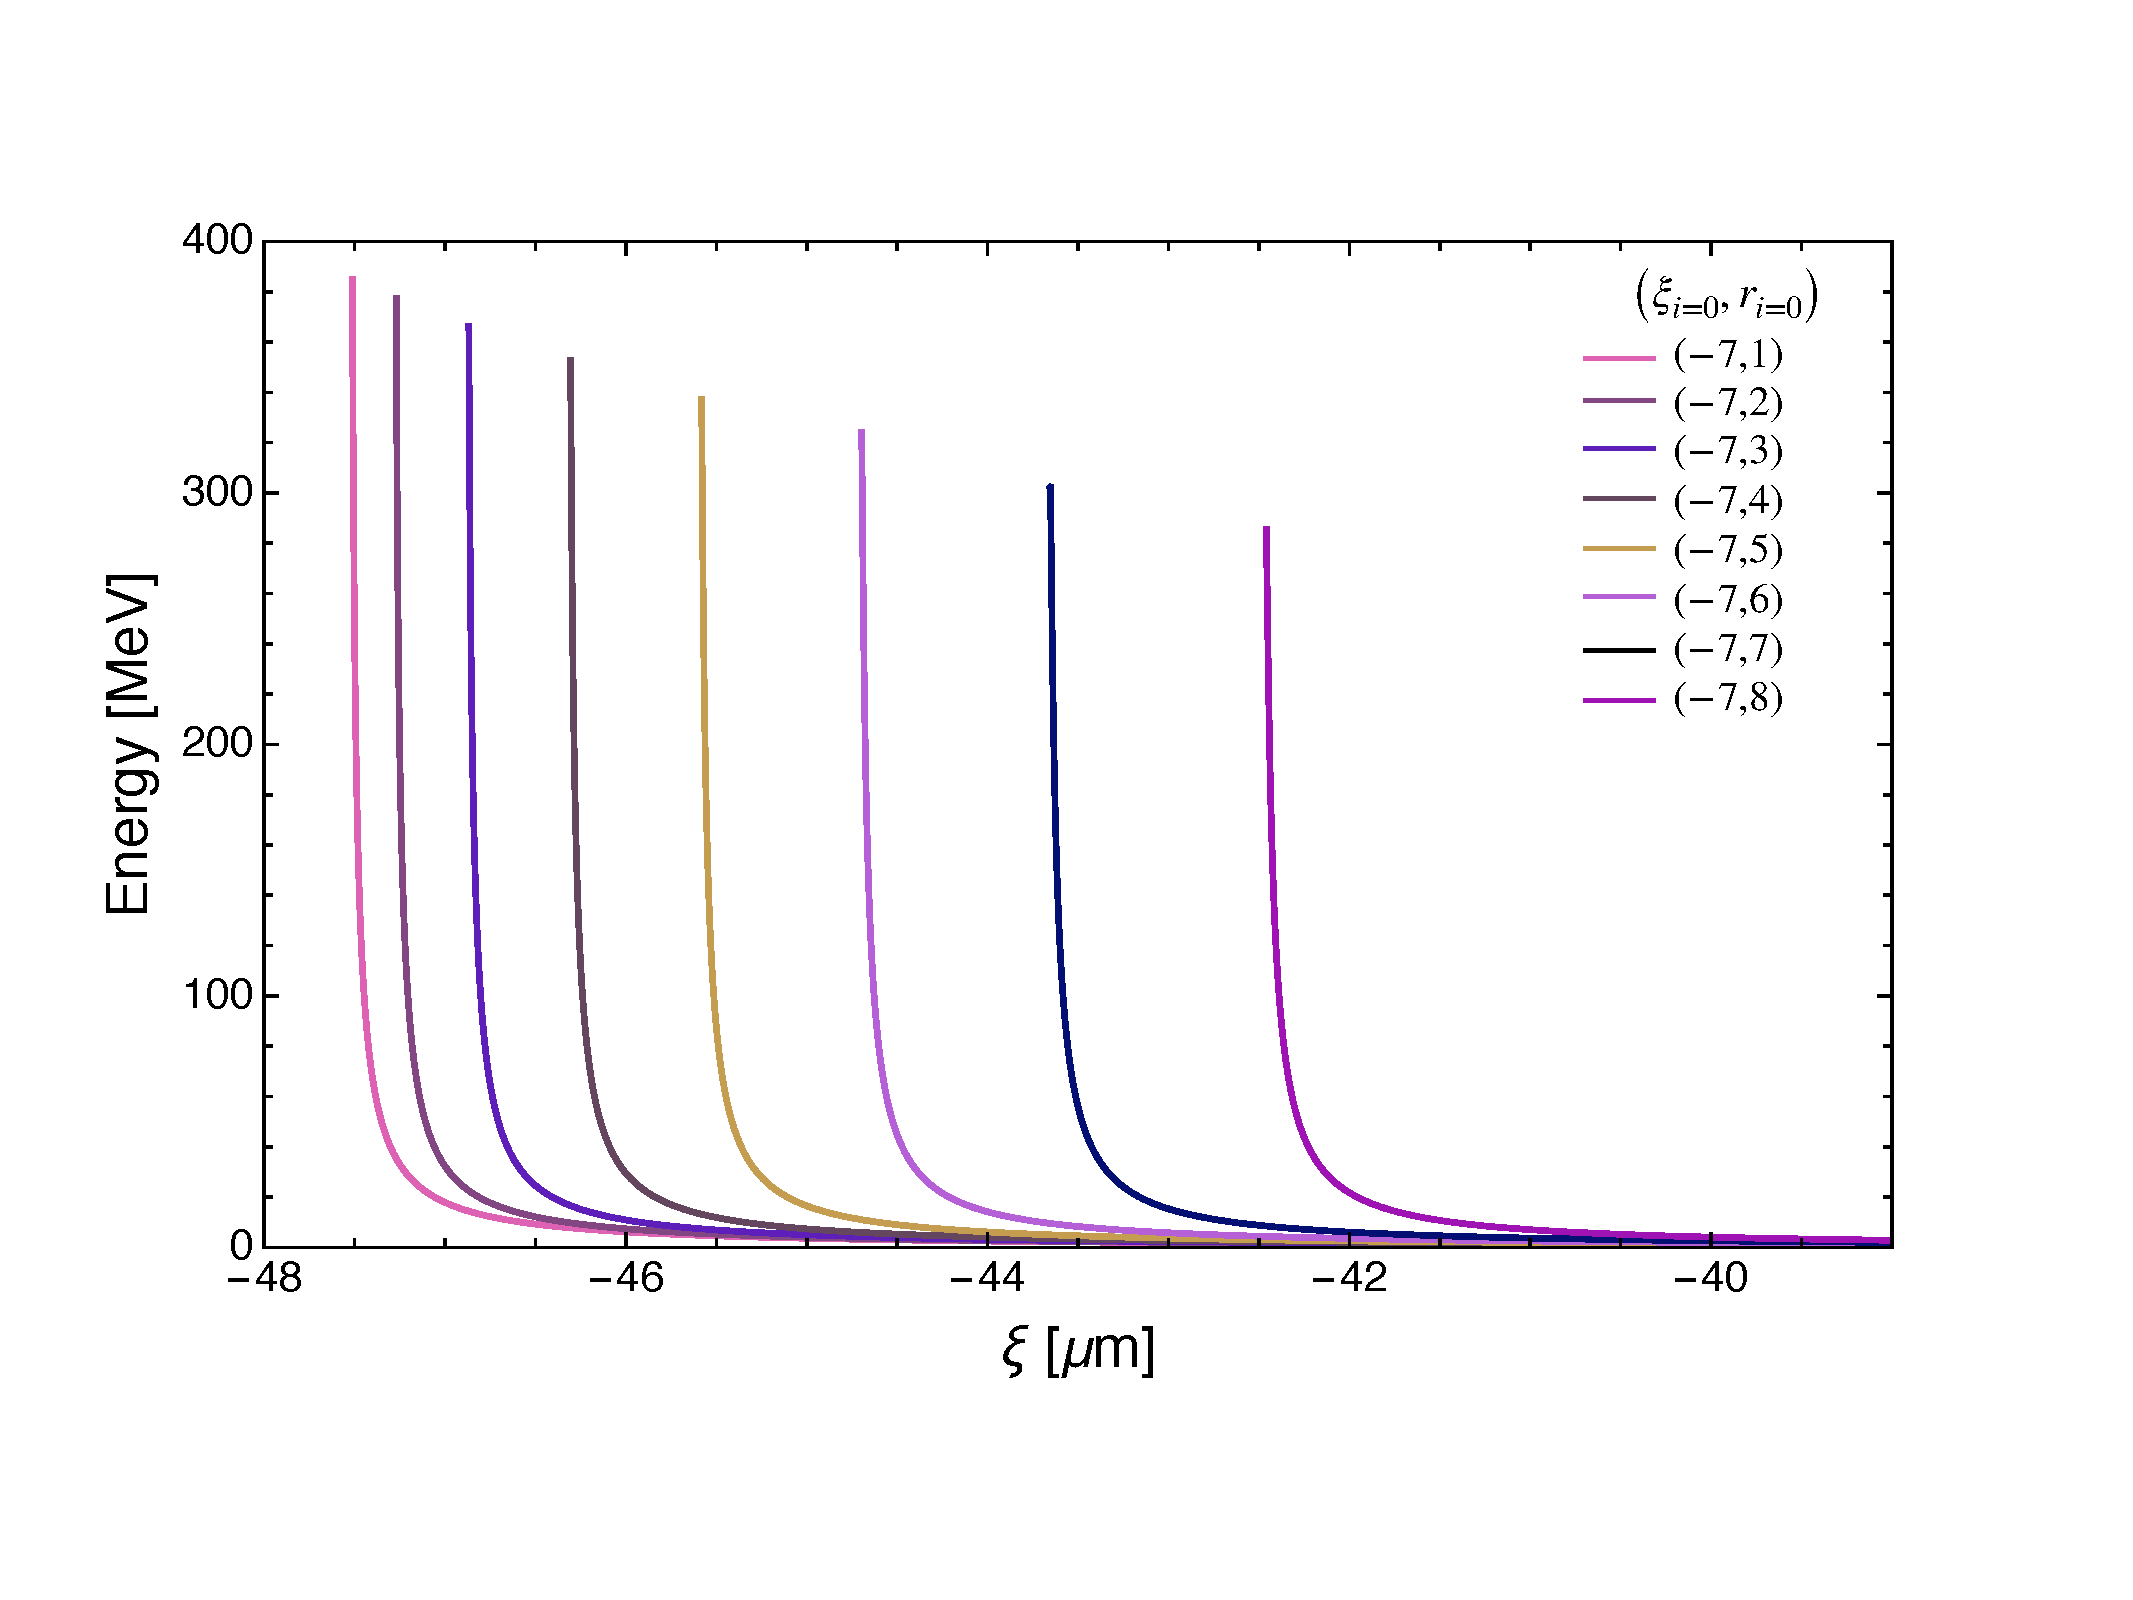
\includegraphics[width=0.7\textwidth]{RadialEnergies}
\caption{Radial energies, xi}
\label{Radial Energies}
\end{figure}
\begin{figure}
\centering
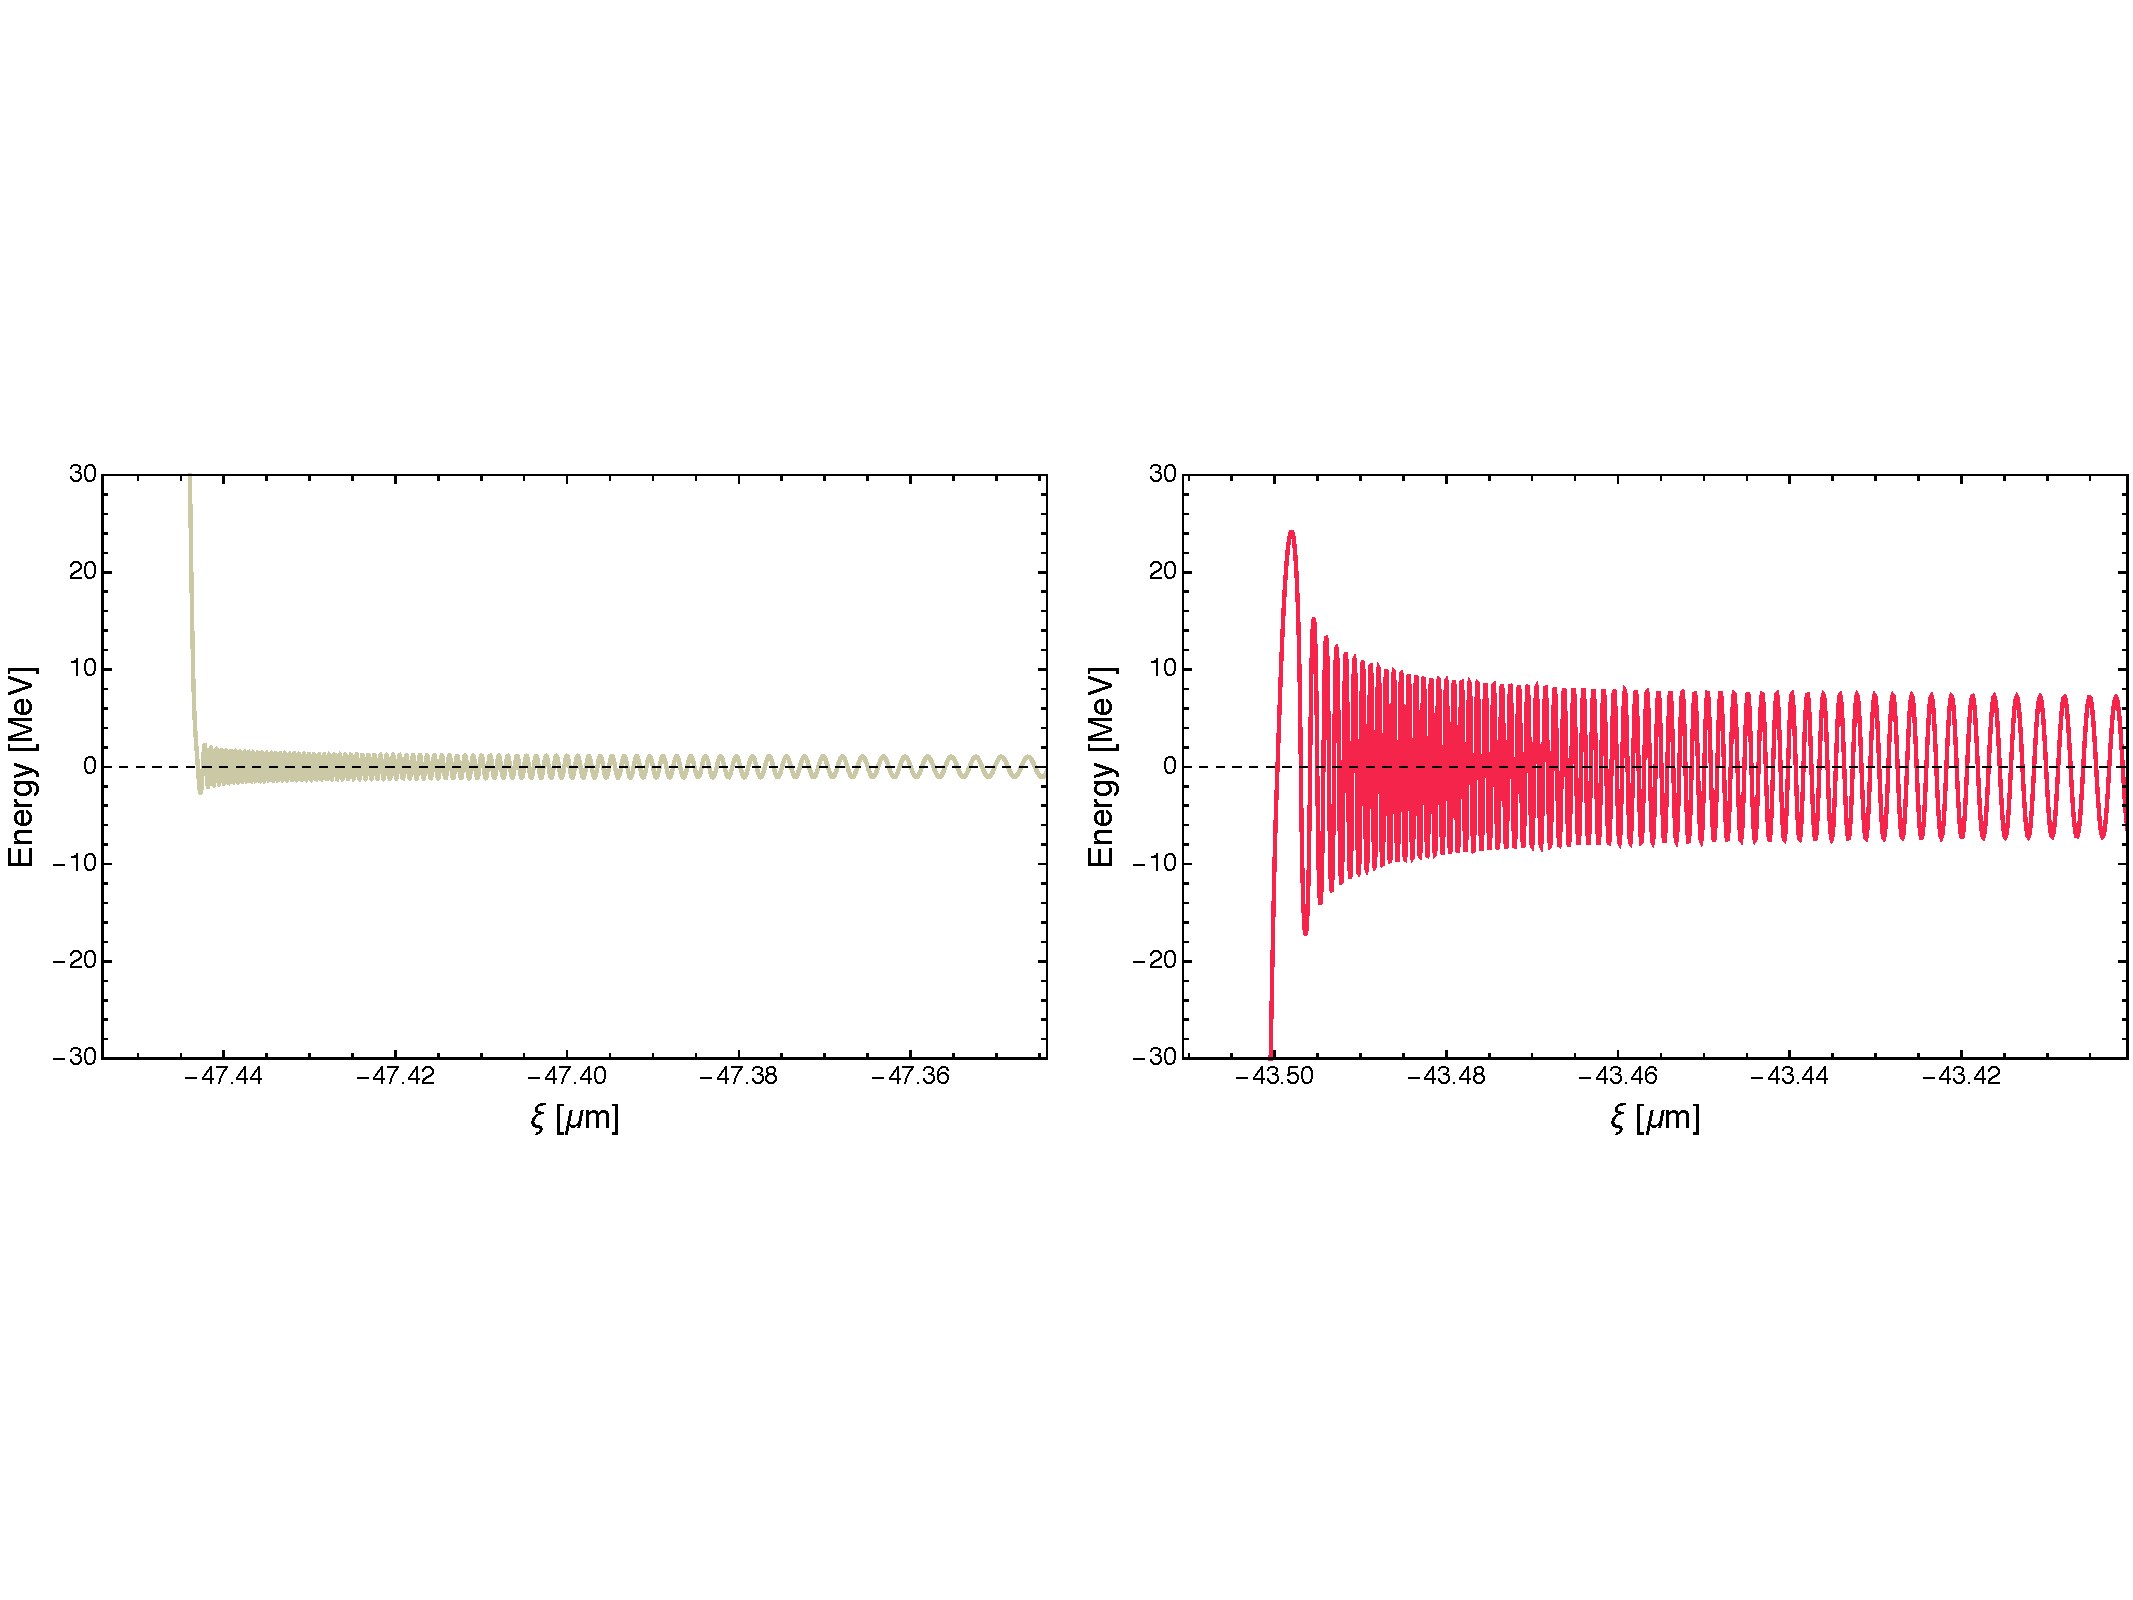
\includegraphics[width=\textwidth]{RadialOscillations}
\caption{abc}
\label{Radial Energies}
\end{figure}

Finally, even if we disregard the high energy of the first set of ejected particles, the total ejected energy in figure XXX is higher in the model than in the simulation. Similar to the beam energy, this is due to the wakefield in our model not weakning as the beam propagates. Since each test particle represetn a volume, this leads to regions of our pseudo-beam getting decelerated to non-realtivistc velocities, and subsequently its particles ejected, at a rate that is higher than the beam in the simulation. For a more accurate model it is clear that we need to address the issue of particle-loss.
\subsection{Dynamic beam density}
The model presented above is able to compute the dynamics of a particle, and by extension the dynamics of a beam, at a reasonable computational time due to the approximations we have used. In particular, the fact that closed-form expressions are found for the wakefield integrals in equations \ref{LongitduinalIntegral} and \ref{transverseIntegral} means that these computationally expensive integrals only need to be evaluated once at the start of the algorithm. The importance of maintaining this feature restricts the range of improvements we can introduced to the model. One of these restrictions is that we can not alter the functional shape of the beam, since this would require re-integration of the wakefields. Instead, we choose to maintain the bi-Gaussian shape of the beam but add a functional dependence to the amplitude of the closed-form expressions for the longitudinal and transverse wakefields. Since we assume the beam shape is constant, this amplitude should only vary due to the total number of particles in the bi-Gaussian part of the beam, since the plasma response from individual particles falling behind is negligible. We therefore need to specify a way of determining when a test-particle has fallen behind the beam. Initial tests were done with strict beam boundaries, whereby the contribution of the $n^\text{th}$ test-particle to the total number of particles was set to zero once it had fallen behind to a position $\xi_{i}^{(n)}<-5\sigma_{\xi}$, for instance. This however lead to successive sharp drops in the amplitude of the wakefield, which in turn induced instabilities in the particles' radial oscillations which ultimately ejected particles before entering the defocusing region. 

to this end, we reduce the influence of each test-particle smoothly 

This is the same as saying that some of the particles that the test-particle represents stay at that positions.

\begin{equation}
N_{\text{chirp}}(z)= \sum_{n=0}^N T_e^{(n)}(z)\times N(\xi_{i=0}^{(n)},r_{i=0}^{(n)})
\end{equation}
where
\begin{equation}
N\left(\xi_{i=0}^{(n)},r_{i=0}^{(n)}\right)=2\pi r_{i=0}^{(n)}\times\Delta r_{i=0}^{(n)}\times\Delta \xi_{i=0}^{(n)}\times\exp[-\frac{\left(\xi_{i=0}^{(n)}\right)^2}{2\sigma_{\xi}^2}-\frac{\left(r_{i=0}^{(n)}\right)^2}{2\sigma_{r}^2}]
\end{equation}
is the relative number of particles that the $n^{\text{th}}$ test-particle represents.
\begin{figure}
\centering
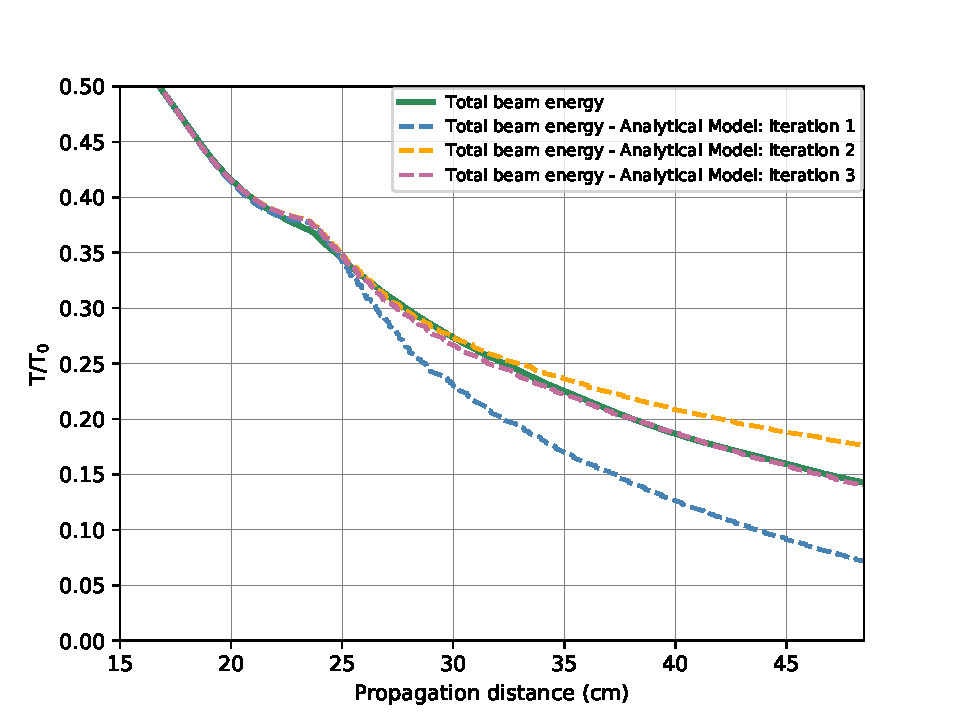
\includegraphics[width=0.52\textwidth]{IterationsEnergy.pdf}\hspace{-25pt}
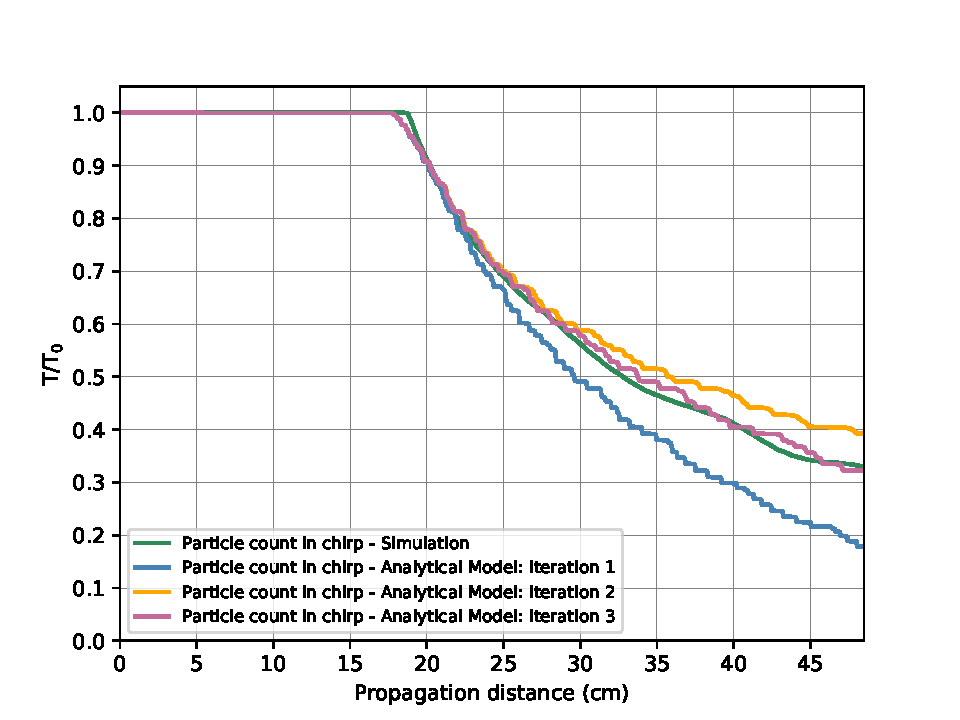
\includegraphics[width=0.52\textwidth]{Particlesinbeamconstant1to102.pdf}
\end{figure}
%This leads us to an interesting line of inquiry: What causes the initial large difference and why does the predicted average energy sti



%This leads us to two important questions. 
%It is interesting that, despite this disparity, the average energy per ejected particle is  


%[Plot of energy of ejected particle w.r.t starting position]\\
%[takj abut total ejected energy, and that this suggests we lose more particles from the beam than in the simualtion, show particle-in-chirp plot and explain how this is calculated, mini-Gaussians etc.]\\
%[Then say that with this plot at hand we can use this to make a simple model of the weakening wakefield]

\newpage
Plot maximum electric field from model and epoch.\\
Add loss of particle calculation and iteration of self-updating of algorithm without having to redo integral for beam density.\\
Use gaussian for particle loss to model that the influence of a particle on the induced wakefield diminshes gradually as it falls through the bunch. Better than sharp particle count cut if fallen behind chirp.




\newpage
\begin{equation}
\label{WApprox}
\begin{split}
W\left(\xi,r,z\right)&=\frac{i e^{-\frac{1}{2} k_p\left(k_p\sigma \xi ^2+2 i \xi \right)}n_{b_0} \sqrt{\frac{\pi }{2}} \sigma \xi  \delta
   \left(r-\sqrt{2} \text{$\sigma $r}\right) \text{erfc}\left(\frac{\xi -i k_p\sigma \xi ^2}{\sqrt{2} \sigma \xi }\right) r^2}{4
   \text{$\sigma $r}^2}\\
   &-\frac{i e^{i k_p\xi -\frac{k_p^2 \sigma \xi ^2}{2}}n_{b_0} \sqrt{\frac{\pi }{2}} \sigma \xi  \delta
   \left(r-\sqrt{2} \text{$\sigma $r}\right) \text{erfc}\left(\frac{i k_p\sigma \xi ^2+\xi }{\sqrt{2} \sigma \xi }\right) r^2}{4
   \text{$\sigma $r}^2}\\
   &+\frac{i e^{-\frac{1}{2} k_p\left(k_p\sigma \xi ^2+2 i \xi \right)}n_{b_0} \sqrt{\frac{\pi }{2}} \sigma \xi
    \delta \left(r-\sqrt{2} \text{$\sigma $r}\right) \text{erfc}\left(\frac{\xi -i k_p\sigma \xi ^2}{\sqrt{2} \sigma \xi
   }\right)}{k_p^2 \text{$\sigma $r}^2}\\
   &-\frac{1}{2} i e^{-\frac{1}{2} k_p\left(k_p\sigma \xi ^2+2 i \xi \right)}n_{b_0}
   \sqrt{\frac{\pi }{2}} \sigma \xi  \delta \left(r-\sqrt{2} \text{$\sigma $r}\right) \text{erfc}\left(\frac{\xi -i k_p\sigma \xi
   ^2}{\sqrt{2} \sigma \xi }\right)\\
   &+i e^{-\frac{1}{2} k_p\left(k_p\sigma \xi ^2+2 i \xi \right)}n_{b_0} \sqrt{\frac{\pi }{2}}\sigma \xi  I_2\left(\sqrt{2} k_p\text{$\sigma $r}\right) K_0(k_pr) \delta \left(r-\sqrt{2} \text{$\sigma $r}\right)\\
   &\text{erfc}\left(\frac{\xi -i k_p\sigma \xi ^2}{\sqrt{2} \sigma \xi }\right)-i e^{-\frac{1}{2} k_p\left(k_p\sigma \xi ^2+2 i
   \xi \right)}n_{b_0} \sqrt{\frac{\pi }{2}} \sigma \xi  I_0(k_pr) K_2\left(\sqrt{2} k_p\text{$\sigma $r}\right) \delta
   \left(r-\sqrt{2} \text{$\sigma $r}\right) \text{erfc}\left(\frac{\xi -i k_p\sigma \xi ^2}{\sqrt{2} \sigma \xi }\right)\\
   &-\frac{i e^{i
   k_p\xi -\frac{k_p^2 \sigma \xi ^2}{2}}n_{b_0} \sqrt{\frac{\pi }{2}} \sigma \xi  \delta \left(r-\sqrt{2} \text{$\sigma $r}\right)
   \text{erfc}\left(\frac{i k_p\sigma \xi ^2+\xi }{\sqrt{2} \sigma \xi }\right)}{k_p^2 \text{$\sigma $r}^2}+\frac{1}{2} i e^{i
   k_p\xi -\frac{k_p^2 \sigma \xi ^2}{2}}n_{b_0} \sqrt{\frac{\pi }{2}} \sigma \xi  \delta \left(r-\sqrt{2} \text{$\sigma $r}\right)\\
   &\text{erfc}\left(\frac{i k_p\sigma \xi ^2+\xi }{\sqrt{2} \sigma \xi }\right)-i e^{i k_p\xi -\frac{k_p^2 \sigma \xi ^2}{2}}
  n_{b_0} \sqrt{\frac{\pi }{2}} \sigma \xi  I_2\left(\sqrt{2} k_p\text{$\sigma $r}\right) K_0(k_pr) \delta \left(r-\sqrt{2}
   \text{$\sigma $r}\right) \text{erfc}\left(\frac{i k_p\sigma \xi ^2+\xi }{\sqrt{2} \sigma \xi }\right)\\
   &+i e^{i k_p\xi
   -\frac{k_p^2 \sigma \xi ^2}{2}}n_{b_0} \sqrt{\frac{\pi }{2}} \sigma \xi  I_0(k_pr) K_2\left(\sqrt{2} k_p\text{$\sigma
   $r}\right) \delta \left(r-\sqrt{2} \text{$\sigma $r}\right) \text{erfc}\left(\frac{i k_p\sigma \xi ^2+\xi }{\sqrt{2} \sigma \xi
   }\right)\\
   &+\frac{i e^{-\frac{1}{2} k_p\left(k_p\sigma \xi ^2+2 i \xi \right)}n_{b_0} \sqrt{\frac{\pi }{2}} \sigma \xi 
   \left(-\text{erf}\left(\frac{\xi -i k_p\sigma \xi ^2}{\sqrt{2} \sigma \xi }\right)-e^{2 i k_p\xi }+e^{2 i k_p\xi }
   \text{erf}\left(\frac{i k_p\sigma \xi ^2+\xi }{\sqrt{2} \sigma \xi }\right)+1\right)}{2 \text{$\sigma $r}^2} \\
   &\frac{\left(\left(2 k_pI_2\left(\sqrt{2} k_p
   \text{$\sigma $r}\right) K_1(k_pr) \text{$\sigma $r}^2+2 k_pI_1(k_pr) K_2\left(\sqrt{2} k_p\text{$\sigma $r}\right)
   \text{$\sigma $r}^2-r\right) \theta \left(\sqrt{2} \text{$\sigma $r}-r\right)\right)}{2 \text{$\sigma $r}^2}\\
   &\frac{\left(-2 k_p\text{$\sigma $r}^2 I_2\left(\sqrt{2} k_p
   \text{$\sigma $r}\right) K_1(k_pr)\right)}{2 \text{$\sigma $r}^2}
   \end{split}
\end{equation}
Radial integral fully simplified
\begin{equation}
\begin{aligned}
&\frac{2 K_0(\text{kp} r) I_2\left(\sqrt{2} \text{kp} \text{$\sigma $r}\right)}{\text{kp}^2}\\
&-\frac{\theta \left(\sqrt{2} \text{$\sigma
   $r}-r\right) \left(\text{kp}^2 \left(r^2-2 \text{$\sigma $r}^2\right)+4 \text{kp}^2 \text{$\sigma $r}^2 \left(K_0(\text{kp} r)
   I_2\left(\sqrt{2} \text{kp} \text{$\sigma $r}\right)-I_0(\text{kp} r) K_2\left(\sqrt{2} \text{kp} \text{$\sigma $r}\right)\right)+4\right)}{2
   \text{kp}^4 \text{$\sigma $r}^2}
   \end{aligned}
\end{equation}

%\begin{equation}
%\frac{K_0(\text{kp} r) \left(\theta \left(\sqrt{2} \text{$\sigma $r}-r\right) \left(-\text{kp} r \left(r^2-2 \text{$\sigma $r}^2\right)
 %  I_1(\text{kp} r)+2 r^2 I_2(\text{kp} r)-4 \text{$\sigma $r}^2 I_2\left(\sqrt{2} \text{kp} \text{$\sigma $r}\right)\right)+4 \text{$\sigma
  % $r}^2 I_2\left(\sqrt{2} \text{kp} \text{$\sigma $r}\right)\right)}{2 \text{kp}^2 \text{$\sigma $r}^2}
%\end{equation}
